% +--------------------------------------------------------------------+
% | Sample Chapter 4 Arquitectura
% +--------------------------------------------------------------------+

\cleardoublepage

\chapter{Epfiot Architecture}
\label{makereference4}

In this chapter, we'll discuss more advanced aspects of Epfiot architecture. To carry out this project, Epfiot main application has been written from scratch, for the bootstrapping service part it was done on the Wakaama implementation as already seen in chapter \ref{makereference3.2.2}.

Epfiot then consists in two separate pieces of software:
\begin{itemize}
    \item \textbf{Epfiot go platform}: Golang Service with the main application.
    \item \textbf{Epfiot bootstrap}:  C - UDP Socket with LwM2M logic.
\end{itemize}

\begin{figure}[h!]%t=top, b=bottom, h=here
\centering
    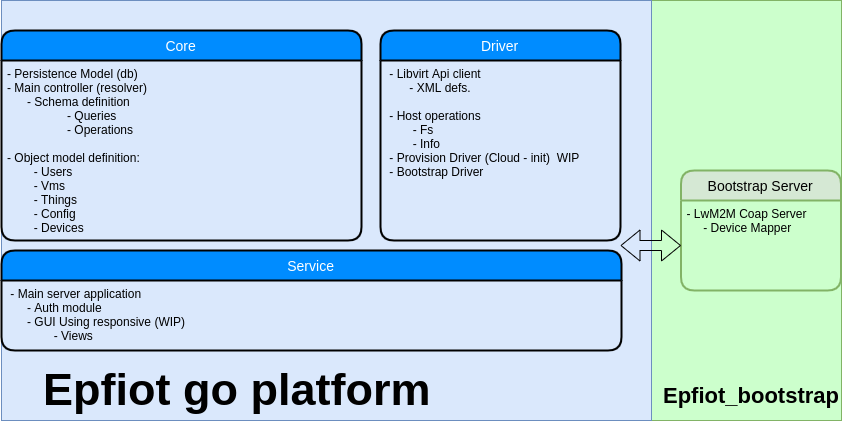
\includegraphics[width=5.5in]{figures/Application.png}
~\caption{Epfiot Overview}
\label{figure4.1}
\end{figure}
The following pages will show the implementation details taken for both parts.



\section{Epfiot platform}
\label{makereference4.2}

The main platform is a program written in Go that makes up most of the Epfiot Service.
It provides the following features:
\begin{itemize}
    \item Modern http API with basic authentication
    \item Sql as data model persistence
    \item Infrastructure management with near baremetal performance with USB passthrough for gpu computing
    \item Basic infra provisioning
    \item IoT oriented
    \item GUI
\end{itemize}

Being a program written from scratch made it necessary to do some architectural work in order to put all the logic together. The result was the creation of some modules differentiated by the function they perform within Epfiot.

\newpage
\subsection{Driver Module}
This module serves as an interface to different functionalities that Epfiot has to deal with, mostly related to host communication or the appliance itself. Some of them are:
\begin{itemize}
    \item \textbf{Virtual machine management}
    \item provisioning
    \item File system and OS operations
    \item Udp Client
\end{itemize}

\begin{figure}[h!]%t=top, b=bottom, h=here
\centering
    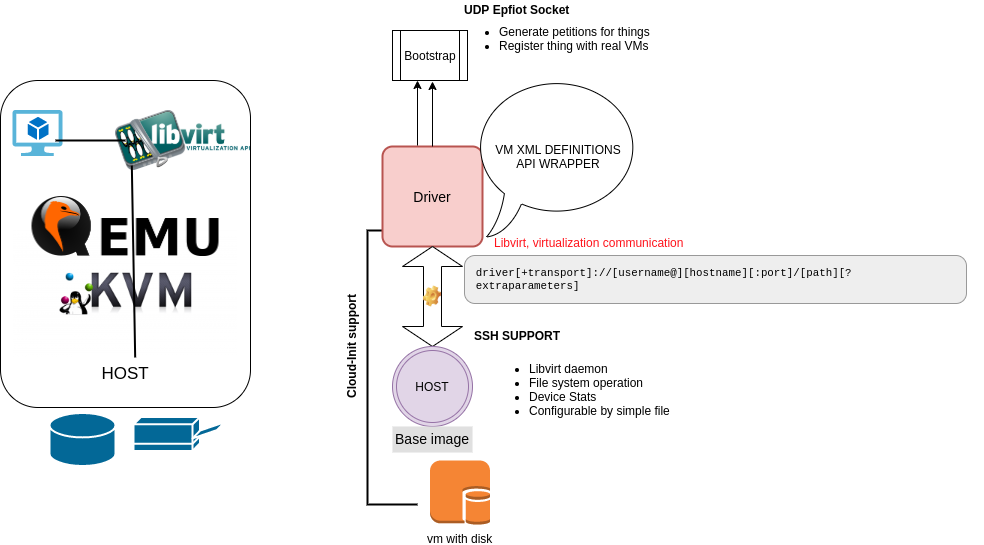
\includegraphics[width=6.0in]{figures/driver.png}
~\caption{Driver module overview}
\label{figure4.2}
\end{figure}

\textbf{Controller}

The protagonist of this module is the infrastructure Controller. This is the part of Epfiot that communicates with the host and handles the virtual machines. To perform this secure communication it uses SSH, which is compatible with Libvirt, the virtualization API with which Epfiot is able to control KVM AND QEMU from the host side.

It is important to know that the Controller is written in a decoupled form and activated by a configuration file, which means that it is possible to write another controller to put it to work with Epfiot!
This decision was made so that the project could evolve into newer forms of virtualization/containers in a near future without changing the rest of the functionality.
To build the Controller, a Golang interface is used in order to allow Epfiot to work with certain infrastructure functionalities that the driver has to implement.
The other Epfiot modules will work using this interface exposed by the controller.

\textbf{System operations} aka \textit{Utils}

With only the controller it is not possible to perform all the operations related to infrastructure. That is why the driver has a number of functions in the form of utilities to support the controller.

This part then takes care of some IO operation such as creating/copying/deleting disks or getting host information.

\textbf{Provisioning}

Epfiot is able to perform some basic provisioning operations. This part of the Driver module takes care or creating CD-ROMS with user settings (available via Epfiot API). This cdrom is inserted into the machine at its deployment and thanks to Cloud-Init it is able to perform actions such as creating users, installing packages, running scripts...

At the moment in Epfiot, the provisioning part only provides with the basic access credentials for the machine user and some basic networking however, is planned to expand the functionality in order to allow more operations.

\textbf{Udp communication}

Finally, the Driver module also handles Epfiot communications related to UDP. This is directly related to the bootstrapping part we'll see later.

The module acts as an UDP client to send certain information to the Epfiot Bootstrap process. This part of the module serves as an interface between Golang and C, something totally mandatory for use LWM2M implementations.

\newpage
\subsection{Service Module}

This section of Epfiot is responsible for serving an interface to the user.
Some of the purposes this module serves are as follows:
\begin{itemize}
    \item Authentication and security
    \item \textbf{ HTTP API endpoint}
    \item GUI
\end{itemize}

\begin{figure}[h!]%t=top, b=bottom, h=here
\centering
    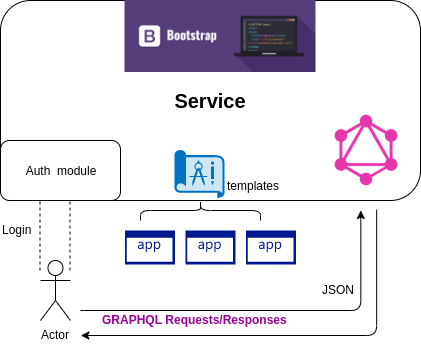
\includegraphics[width=4.0in]{figures/Service.png}
~\caption{Service module overview}
\label{figure4.3}
\end{figure}

\textbf{Epfiot API}

This module is responsible for exposing the operation api to the user.
Use Golang "net/http" native library to provide a fast we service. As you know, this module instead of using REST takes another perspective using a Graphql framework. This allows Epfiot to have a single endpoint where it is able to expose all operations through one schema. This scheme is described in Chapter \ref{makereference5.1}.

The user being aware of this scheme, is able to send json as a console to interact with Epfiot. This endpoint will respond with json objects depending on what the user asks.
\newpage

\textbf{Authentication}

Epfiot is a multitenant application, which means that it is capable of registering user and interacting with them. For this reason it is necessary to authenticate with Epfiot. 
The service module handles this authentication by maintaining a secure session for the user.

In the current version of Epfiot only a basic version of this module is implemented which allows you to identify the user and maintain their session.

\textbf{GUI}

To finish with this module we come to the part of the visual interface. The module has a visual system using the html/css/javascript templates offered by golang.

At the moment the most functional part of this visual interface is the console however, The logic that covers the rendering code is working and it is possible to make some graphic windows in a very simple way.



\newpage
\subsection{Core}

Core is the most fundamental part of Epfiot. The Epfiot Core can be understood as the heart of the application. In this module we find the code that controls the other modules (like the one for the Driver). In addition, the object model governing the entire application is defined here.

Some of the functions that this module performs are:
\begin{itemize}
    \item Objects definition (model)
    \item Database layer for model persistence
    \item Manage the data flow/operations of the entire application
\end{itemize}

\begin{figure}[h!]%t=top, b=bottom, h=here
\centering
    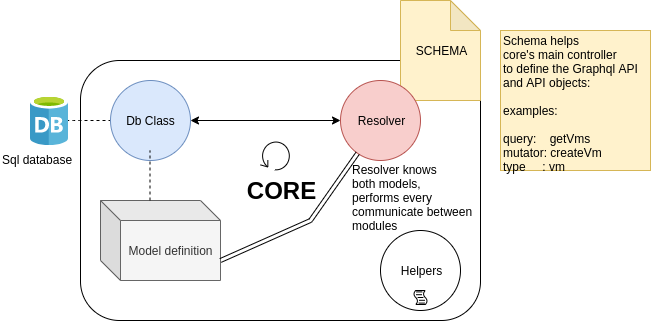
\includegraphics[width=5.5in]{figures/Core.png}
~\caption{Core overview}
\label{figure4.4}
\end{figure}

\textbf{Resolver}

Resolver is the class that handles the application. This code is in charge of receiving the actions dictated by the user through graphql, it is capable of of calling other modules to perform concrete actions. Inside this controller we can find many data definitions that the user is able to use in first instance (Chapter \ref{makereference5.1.1}).

As a design decision, Resolver save a pointer to the instance of the Driver module with which Epfiot is running.
As mentioned, Epfiot's architecture is decoupled and although at the moment there is only one driver for KVM, it is possible to implement any other as long as you keep the interface.


When the user makes an API call such as createVm, Epfiot uses the service module to handle any http session, right after that Resolve dictate what action to take.

\begin{figure}[h!]%t=top, b=bottom, h=here
\centering
    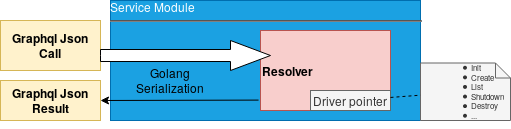
\includegraphics[width=5.0in]{figures/resolver.png}
~\caption{Service - Resolver - Driver Flow}
\label{figure4.5}
\end{figure}

\textbf{Data persistence}

As expected, one of the most important parts of the core is data persistence. Epfiot uses a relational model to store data and infrastructure status. To take this process, Core has a class that is exclusively in charge of communicate with the database.

When changes are made to the model, Resolver is able to access this storage layer in order to allow data persistence.

\textbf{Epfiot Model}

We refer to the model as the series of defined objects and the relationships they form with each other that Epfiot offers to the user in order to manage the infrastructure and IoT environment.

These objects that we can find inside Epfiot are the following:
\begin{itemize}
    \item \textbf{User}: The normal user entity that uses the application to know who own the environment.
    \item \textbf{Vm}: Representing the infrastructure, keeping information about the details of the machine and the status.
    \item \textbf{Devices}: Each of these objects represents the usb devices that has attached, storing information such as the bus number.
    \item \textbf{Things}: They represent the various IoT sensors you deploy and their relationship to the infrastructure.
    \item Config: The only purpose of this object is to save instance initialization options that could be reused.
\end{itemize}
\newpage

As you can see, the Epfiot model is quite simple and useful for the user to build his environment without any headache.


\begin{figure}[h!]%t=top, b=bottom, h=here
\centering
    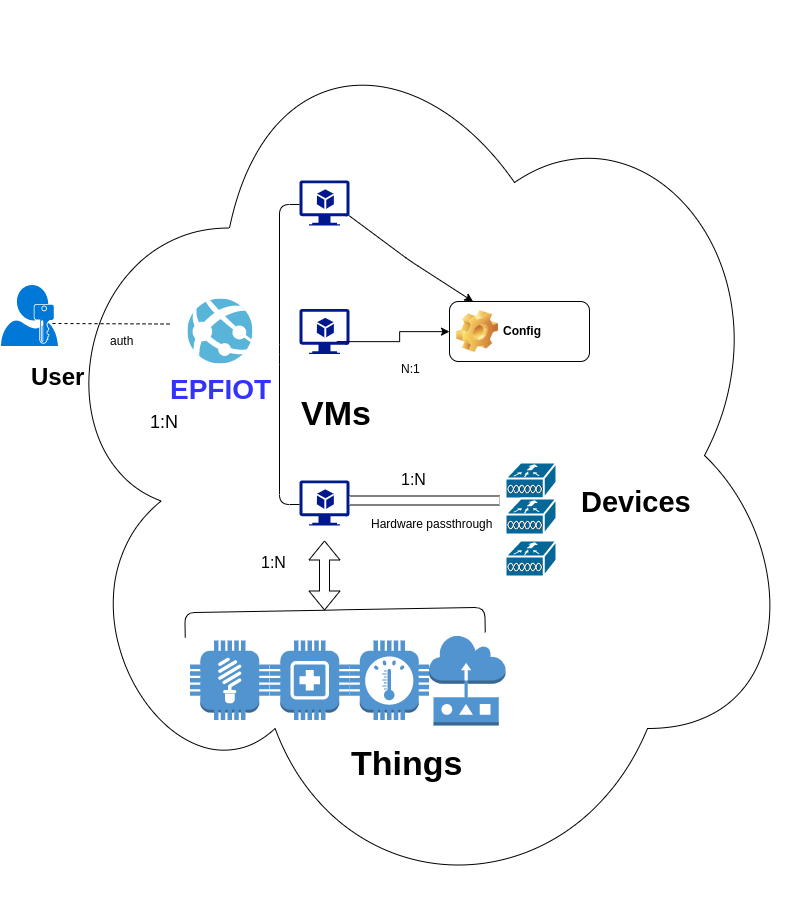
\includegraphics[width=6.0in]{figures/core_model.png}
~\caption{Epfiot Model Overview}
\label{figure4.6}
\end{figure}
\newpage


\section{Epfiot Bootstrap}
\label{makereference4.3}
In the Core part we have seen the underlying model of the application \ref{makereference4.2}. Specifically, there's part of this model called "things".
These objects not only serve to store information, but must actually be related to real sensors. To interact with those sensors it was decided the use of lwm2m2 protocol, an application layer for IoT device management.

Integrating Lwm2m2 into Epfiot was not an easy task, is a young protocol and there are still not many written implementations to use.
Finally Epfiot\_bootstrap was born a 'separate' project made for meet the requirements of lwm2m2 and take advantage of Eclipse Foundation's Wakaama implementation.

This part of Epfiot as its name suggest is based on the bootstrap service provided by lwm2m. A service with this implementation is launched in parallel to the main platform. A service with this implementation is launched in parallel to the main platform in charge of establishing relationships between the vms and the things.

\begin{figure}[h!]%t=top, b=bottom, h=here
\centering
    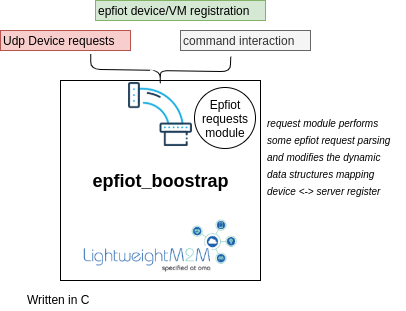
\includegraphics[width=5.0in]{figures/bootstrap.png}
~\caption{Epfiot\_bootstrap Overview}
\label{figure4.7}
\end{figure}

This process is listens to UDP packets and stores in memory the bootstrapping configuration for different sensors.
\newpage

Some of the actions performed by Epfiot bootstrap are the next:
\begin{itemize}
    \item Has implemented a protocol on udp built for Epfiot
    \item Store information about Epfiot vms and things
    \item When a sensor asks for bootstrapping configuration, Epfiot is able to configure it using its internal model
    \item Notify the main Platform that a client (sensor) has been registered and associated with certain vm
\end{itemize}

\begin{figure}[h!]%t=top, b=bottom, h=here
\centering
    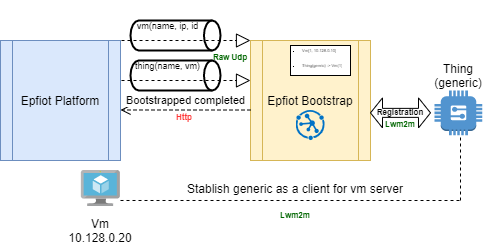
\includegraphics[width=6.5in]{figures/Epfiot_bootstrap_example.png}
~\caption{Epfiot\_bootstrap example}
\label{figure4.8}
\end{figure}

